\section{Aufbau}
\label{sec:Aufbau}
Der Versuchsaufbau zur Messung eine Franck-Hertz-Kurve ist in Abbildung \ref{fig:aufbau} dargestellt.
Er besteht aus der Franck-Hertz-Apparatur, deren Kathode über eine Konstantstromquelle aufgeheizt werden kann.
Des Weiteren gibt es noch eine Heizstromquelle zur Regelung Temperatur im Glaskolben, welche über ein Thermometer abgelesen werden kann. Eine regelbare Gleichstromquelle erzeugt eine Beschleunigungsspannung $U_.B$ von bis zu $\SI{60}{\volt}$ und eine Bremsspannung $U_.A$ von bis zu $\SI{10}{volt}$ und kann mit der X-Komponente des XY-Schreibers verbunden werden. Die Auffangelektrode wird an ein Amperemeter angeschlossen welches den ankommenden Strom anzeigt und mit der Y-Komponente verbunden ist. Außerdem gibt es noch eine Konstantspannungsquelle, die eine Bremsspannung von $\SI{30}{\volt}$ liefert.

\begin{figure}
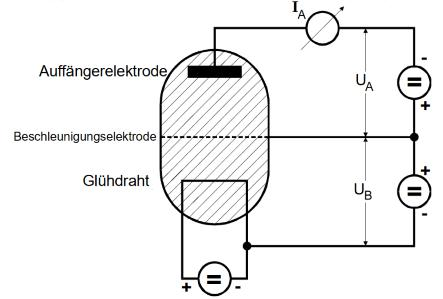
\includegraphics[width=\linewidth-50pt,height=\textheight-50pt,keepaspectratio]{content/images/apparatur.jpg}
\caption{Schematischer Versuchsaufbau zur Bestimmung der Ionisations- und ersten Anregungsenergie des Hg-Atoms \cite{V601}.}
\label{fig:aufbau}
\end{figure}
